\cotefile{1}
\scanpage{122}
\[
n!\alpha_n\leq\frac{\varepsilon_0}{n+1}\,
\varepsilon_1\mathord{-}\mathord{-}\varepsilon_n\,e^n
\qquad
\sqrt[n]{n!\alpha_n}\leq e\left(\frac{\varepsilon_0}{n+1}\right)^{1/n}
\deleted{\unsure{\varepsilon_1\ldots\varepsilon_n}}
\inserted{(\varepsilon_1\mathord{-}\varepsilon_n\unsure{,}}
\]
$\unsure{(}n\to\infty$,
$\left(\frac{\varepsilon_0}{n+1}\right)^{1/n}\to1$, and
$(\varepsilon_1\mathord{.}\mathord{.}\varepsilon_n)^{1/n}\to0$,
as one sees immediately, whence $\sqrt[n]{n!\alpha_n}\to0$,
whence it follows that $\sum n!\alpha_n(\lambda)$ converges absolutely
\unsure{$\lambda$|at}. It follows from this
\margin{\unsure{for every subspace|on every subspace} of finite dimension $\unsure{F|E}\unsure{\subset|\text{of}}l^1$,
the function $S(\lambda)$ is holomorphic
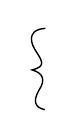
\begin{tikzpicture}[x=.008cm,y=.008cm]
\draw[line width=.5pt] (30,129) .. controls (7,128) and (3,113) .. (13,96)
.. controls (25,77) and (32,69) .. (9,63)
.. controls (26,58) and (31,48) .. (20,31)
.. controls (10,14) and (13,3) .. (29,0);
\end{tikzpicture}}

Since we have $|\alpha_n(\lambda)|\leq\|\lambda\|_1^n$, it follows that
the function $S(\lambda)$ \inserted{on $l^1$}
\begin{tikzpicture}[x=.012cm,y=.012cm,baseline=-.3ex]
\draw[line width=.45pt] (64,65) .. controls (77,54) and (61,41) .. (34,36)
.. controls (13,34) and (8,25) .. (4,0);
\end{tikzpicture}
is holomorphic in a neighborhood
of the origin\,; moreover, the $n$-linear form
$\alpha_n(\lambda^{(1)},\mathord{-},\lambda^{(n)})$ associated with
$\lambda\to\alpha_n(\lambda)$ is
\[
\alpha_n(\lambda^{(1)}\unsure{\mathord{.}\mathord{.}|\ldots}\lambda^{(n)})
=\frac{1}{n!}\sum_{i_1,\mathord{-},i_n}
\lambda^{(1)}_{i_1}\mathord{.}\mathord{-}\lambda^{(n)}_{i_n}
\]
(the sum being taken over the systems $(i_1\mathord{-}i_n)$ of distinct indices)
whence $\|\alpha_n\|\leq\frac{1}{n!}$
\inserted{that is $\unsure{\|}\deleted{\unsure{\alpha_n}}n!\alpha_n\|\leq1$}
\begin{tikzpicture}[x=.018cm,y=.018cm,baseline=-.5ex]
\draw[line width=.45pt] (0,0) .. controls (4,12) and (10,18) .. (16,19)
-- (85,19) .. controls (100,19) and (105,24) .. (106,27);
\end{tikzpicture},
the radius of convergence
in the strict sense \inserted{$R_0$} of the function $S(\lambda)$ at the origin is
therefore \deleted{\unsure{$R_0$|be|à peu}} $\geq1$.
Let \inserted{then} $a_{\deleted{\unsure{m}}}^{(m)}$ be the element of $l^1$
\deleted{\unsure{equal to}} given by
\[
a_i^{(m)}=\begin{cases}
\frac{1}{m}&\text{if }i\leq m\\
0&\text{if }i>m
\end{cases}
\]
we manifestly have $\|a^{(m)}\|_1=1$, and
\[
\alpha_n(a^m)=\deleted{\unsure{\frac{1}{m^n}}}
\left\{\begin{aligned}
&\deleted{\unsure{0\quad\text{if }n>m}}\\
&\frac{1}{m^n}\frac{m!}{n!(m-n)!}\quad\text{if }n\leq m
\end{aligned}\right.\,,\quad\text{whence}
\]
\[
n!\alpha_n(a^m)=\frac{1}{m^n}\,m(m-1)\mathord{-}(m-n+1)
=\unsure{\deleted{1}|\lbrace}
(1-\tfrac{1}{m})(1-\tfrac{\unsure{3|2}}{m})
\mathord{.}\mathord{-}(1-\tfrac{n-1}{m})
\]
Thus $n!\alpha_n(a^{(m)})\to1$ for $m\to\infty$.
It follows that $S(a^{(m)})\to\infty$ if $m\to\infty$ ;
thus $S(\lambda)$ is not bounded in the ball
of unit radius in $l^1$, and its radius of convergence
in the broad sense \inserted{$R_1$} at the origin is therefore also $\leq1$, whence $R_0=R_1=1$.

\deleted{Finally, $S(\lambda)$ being holomorphic in a neighborhood of
\unsure{$0$|$a$} and being able to be \unsure{holomorphic|extended|holomorphic}
on \unsure{each line}}
\margin{123}
